Sikteeri on vuosien varrella paisunut yleiseksi toiminnanohjausjärjestelmäksi, jonka arkkitehtuuria kehittäjät haluaisivat viedä palvelusuuntautuneiden arkkitehtuurien suuntaan, jotta yksittäisten palveluiden kehittäminen olisi kevyempää. Jotta Sikteerin ulkopuolisten web-palveluiden kehittäminen on mahdollista, täytyy erillisillä palveluilla olla tapa tunnistaa käyttäjä. Varsinainen käyttäjähallinta on tällä hetkellä Sikteerin ulkopuolisessa LDAP-tietokannassa, jota vasten Sikteeri tunnistaa käyttäjät. Nykyistä LDAP-tietokantaa halutaan käyttää myös jatkossa keskitetyssä tunnistautumispalvelussa, mutta Sikteerin (tai muun vastaavan palvelun) ei tarvitse päästä suoraan LDAP-kantaan käsiksi.

Sikteeri on Kapsi ry:n laskutuksen ja jäsenhallinnan tarpeisiin kehitetty web-palvelu. Sikteeriin on pääsy Kapsi ry:n hallituksella, ylläpidolla ja ryhmään laskutus kuuluvilla jäsenillä. Lisäksi yhdistyksellä on käytössään erillinen komentorivityökalu, nimeltä admtool, jolla voidaan tehdä erilaisia ylläpitotehtäviä.

Sekä Sikteeri että admtool käyttävät ulkoisena komponenttina LDAP-käyt\-tä\-jä\-hal\-lin\-taa, josta tarkistetaan onko käyttäjällä oikeuksia käyttää kyseisiä palveluita. Nykyinen arkkitehtuuri on kuvattu kuvassa \ref{kapsi_nykyinen}. Kuvaan on lisätty myös suunnitteilla oleva käyttäjien palvelunhallinta, jota kautta jäsenet voisivat lisätä itselleen jäsenmaksuun kuuluvia palveluita, kuten sähköpostialiaksia ja domaineja. Myös käyttäjien palvelunhallinnan tarvitsee tunnistaa käyttäjät, joten nykyisessä arkkitehtuurissa myös sen täytyy integroitua LDAP-käyttäjänhallintaan.

\begin{figure}[h]
\centering
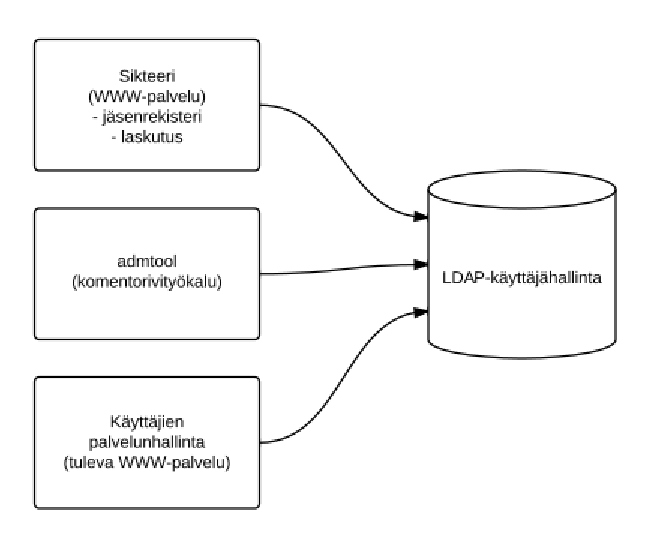
\includegraphics[width=.7\textwidth]{toteutus/kapsi_nykyinen.eps}
\caption{Kapsin jäsenhallintapalveluiden arkkitehtuuri.}%
\label{kapsi_nykyinen}
\end{figure}

Nykyisellään Sikteeri käyttää Django-ohjelmistokehyksen tarjoamaa väliohjelmistoa tunnistautumiseen. Django.contrib.auth-niminen väliohjelmisto tarjoaa hyvät laajentamismahdollisuudet \cite{django_auth}. Siinä on mahdollista määritellä eri taustajärjestelmiä (backend), joita käytetään tunnistautumisessa. Sikteeri käyttää tunnistautumiseen Djangon tarjoamaa ModelBackend-taustajärjestelmää, joka mahdollistaa käyttäjän tunnistautumisen vertaamalla käyttäjän syöttämää käyttäjätunnusta ja salasanaa tietokantaan tallennettuihin käyttäjiin \cite{django_auth}. Jos oikealla tunnus/salasana-parilla oleva käyttäjä löytyy, palautetaan se sovellustasolle.